\documentclass[9pt]{beamer}

\usepackage[utf8]{inputenc}
\RequirePackage[francais]{babel}
%\usepackage{url}
%\usepackage{etex}
%\usepackage{enumitem}
%\usepackage{multicol}
\usepackage{xcolor}
%\usepackage{bbm}
%\usepackage{amsmath,amsthm,amssymb}
%\usepackage[official]{eurosym}
%\usepackage{pifont}
%\usepackage{exercise}
%\usepackage{graphics}
%\usepackage{array,multirow,makecell}
\usepackage{verbatim}
%\usepackage[dvipsnames]{pstricks}
\usepackage{pstricks-add,pst-plot,pst-text,pst-tree,pst-eps,pst-fill,pst-node,pst-math,pst-blur,pst-func}
%\usepackage{pgf,tikz}
%\usepackage{tipfr}
%\usepackage{thmbox}
%\usepackage{calc}
%\usepackage{ifthen}
%\usepackage{pdfpages}
%\usepackage{colortbl}
%\usepackage{sagetex}
%\usetikzlibrary{arrows,patterns}
%\input tabvar
%\usepackage{tkz-tab}
%\usepackage{listings}
%\usepackage[np]{numprint}
%\usepackage{fancybox,fancyhdr}
%\usepackage{thmtools}
%\usepackage{bclogo}
%\usepackage{lastpage}

\usepackage{tabularx}
\usepackage{array,multirow,makecell}
\usetheme{Madrid}
%\usetheme{Bergen}
\usecolortheme{beaver}
 
%Information to be included in the title page:
\title{Python}
\subtitle{Structure de données de base}
\author{Yannick CHISTEL}
\institute{Lycée Dumont d'Urville - CAEN}
\date{Octobre 2020}
 
%----------------------------------------------------------------------------------------------- 
% 							Commandes Tableaux
%-----------------------------------------------------------------------------------------------
\setcellgapes{1pt}
\makegapedcells
\newcolumntype{R}[1]{>{\raggedleft\arraybackslash }b{#1}}
\newcolumntype{L}[1]{>{\raggedright\arraybackslash }b{#1}}
\newcolumntype{C}[1]{>{\centering\arraybackslash }b{#1}}


\newcounter{num}
\setcounter{num}{0}
 
\begin{document}
 
\frame{\titlepage}

\begin{frame}
\frametitle{Les fonctions en Python}

\begin{block}{Présentation}
Une fonction rassemble sous un même nom une séquence d'instructions qui seront exécutées lors de l'appel de la fonction. \medskip

La fonction est introduite par le mot clé \textbf{def} suivi du nom de la fonction, suivi de parenthèses et les deux points qui imposeront une indentation.
\begin{itemize}
\item \textbf{def} nom de la fonction():
\end{itemize}
\end{block}

\begin{block}{Renvoyer un résultat}
Une fonction peut \textbf{renvoyer} ou retourner une valeur. Le mot-clé utilisé en Python pour renvoyer une valeur est \textbf{return}.
\begin{itemize}
\item \textbf{def} nom de la fonction():\\
\hspace{0.5cm} instructions\\
\hspace{0.5cm} \textbf{return} valeur
\end{itemize}
\end{block}
\end{frame}


\begin{frame}
\frametitle{Les fonctions en Python}
\begin{exampleblock}{Exemple}
On veut afficher un carré de 5 colonnes et 5 lignes rempli par la lettre X.\medskip

La fonction \textbf{dessinecarre()} renvoie une chaine de caractères (type string) qui affichera le carré avec la commande \textbf{print}.\medskip

\begin{minipage}{0.6\textwidth}
\includegraphics[scale=0.6]{img/diapoFonction1.eps}
\end{minipage}
\begin{minipage}{0.35\textwidth}
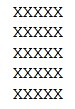
\includegraphics[scale=0.7]{img/carre5X.eps}
\end{minipage}\medskip

L'appel de la fonction \textbf{dessinecarre} provoquera l'exécution de toutes les instructions contenues dans la fonction et renvoie une chaine de caractères contenant des X et des retours à la ligne.
\end{exampleblock}
\end{frame}

\begin{frame}
\frametitle{Les fonctions en Python}

\begin{block}{Fonction avec 1 paramètre}
La fonction précédente \textbf{dessinecarre} réalise des carrés de côté 5. On peut modifier cette valeur en transmettant un \textbf{paramètre} à la fonction. La syntaxe est la suivante :
\begin{itemize}
\item \textbf{def} nom de la fonction(\textbf{paramètre}):\\
\hspace{0.5cm} instructions
\end{itemize}
\end{block}

\begin{exampleblock}{Exemple}
\begin{minipage}{0.75\textwidth}
\includegraphics[scale=0.55]{img/diapoFonction2.eps}
\end{minipage}
\begin{minipage}{0.2\textwidth}
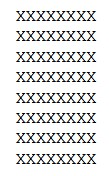
\includegraphics[scale=0.6]{img/carre8X.eps}
\end{minipage}\medskip

L'appel de la fonction \textbf{dessinecarre(8)} réalise un carré de 8 lignes et 8 colonnes.
\end{exampleblock}

\end{frame}

\begin{frame}
\frametitle{Les fonctions en Python}

\begin{block}{Fonction avec plusieurs paramètres}
On peut passer plusieurs paramètres à une fonction selon la syntaxe suivante:
\begin{itemize}
\item \textbf{def} nom de la fonction(\textbf{paramètre1,paramètre2,...}):\\
\hspace{0.5cm} instructions
\end{itemize}
\end{block}

\begin{exampleblock}{Exemple}
\begin{minipage}{0.75\textwidth}
\includegraphics[scale=0.55]{img/diapoFonction3.eps}
\end{minipage}
\begin{minipage}{0.2\textwidth}
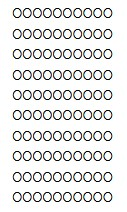
\includegraphics[scale=0.6]{img/carre10O.eps}
\end{minipage}\medskip

L'appel de la fonction \textbf{dessinecarre(10,"O")} réalise un carré de 10 lignes et 10 colonnes avec la lettre O.
\end{exampleblock}

\end{frame}


%\begin{frame}
%\frametitle{Les fonctions en Python}
%
%
%\begin{exampleblock}{Exemple}
%Fonction qui calcule et renvoie la somme des nombres passés en paramètres.
%\begin{itemize}
%\item \textbf{def} somme(a,b,c):\\
%\hspace{0.5cm}s=a+b+c\\
%\hspace{0.5cm}\textbf{return} s
%\end{itemize}
%L'appel de la fonction \textbf{somme} retourne un nombre qui pourra être affecté à une variable.
%\begin{itemize}
%\item x=somme(1,2,3)\\
%\hspace{0cm}print(x)\hspace{3cm}\textit{qui affichera 6.}
%\end{itemize}
%\end{exampleblock}
%
%\end{frame}


\begin{frame}
\frametitle{Les fonctions en Python}

\begin{block}{Variable locale à une fonction}
Une fonction peut utiliser des variables nécessaires à son fonctionnement, pour réaliser des calculs intermédiaires. Ces variables sont dites locales à la fonction.

Il n'est pas possible d'accéder à la valeur d'une variable locale en dehors de la fonction.
\end{block}

\begin{exampleblock}{Exemple}
Fonction qui calcule et renvoie la moyenne des nombres passés en paramètres.
\begin{itemize}
\item \textbf{def} moyenne(a,b,c):\\
\hspace{0.5cm}s=a+b+c\\
\hspace{0.5cm}\textbf{return} s/3
\end{itemize}
\end{exampleblock}

\begin{alertblock}{Attention}
La fonction moyenne utilise une variable locale \textbf{s}. Cette variable n'est pas accessible sauf dans la fonction.
Si on veut afficher la valeur de s avec \textbf{print(s)}, une erreur est affichée !
\end{alertblock}
\end{frame}

\begin{frame}
\frametitle{Les fonctions en Python}

\begin{block}{Interruption d'une fonction}
Il est possible d'arrêter l'exécution d'une fonction en renvoyant une valeur booléenne (True, False). Le mot clé \textbf{return} est présent à plusieurs endroits dans le code de la fonction.
\end{block}

\begin{exampleblock}{Exemple}
La fonction ci-dessous contient une instruction print. L'affichage ne se réalisera pas cas la fonction renvoie un booléen avant l'instruction print.

\begin{center}
\includegraphics[scale=0.6]{img/diapoFonction4.eps}
\end{center}

Dès qu'une condition est vérifiée, l'exécution de la fonction est arrêtée et la valeur booléenne est renvoyée.
\end{exampleblock}
\end{frame}

\end{document}

